\documentclass[12pt]{article}

\addtolength{\textwidth}{1.3in}
\addtolength{\oddsidemargin}{-.65in} %left margin
\addtolength{\evensidemargin}{-.65in}
\setlength{\textheight}{9in}
\setlength{\topmargin}{-.5in}
\setlength{\headheight}{0.0in}
\setlength{\footskip}{.375in}
\renewcommand{\baselinestretch}{1.0}
\renewcommand{\thesection}{\Roman{section}} 
\renewcommand{\thesubsection}{\thesection.\Roman{subsection}}
\linespread{1.5}

\usepackage[pdftex,
bookmarks=true,
bookmarksnumbered=false,
pdfview=fitH,
bookmarksopen=true]{hyperref}
\usepackage[pdftex]{graphicx}
%\usepackage{pdfpages}

\usepackage[usenames,dvipsnames,svgnames,table]{xcolor}
\usepackage{cite}
\usepackage{times, verbatim,bm,pifont,pdfsync}
%\usepackage[hang,flushmargin]{footmisc}%unindents footnotes

% disables chapter, section and subsection numbering
%\setcounter{secnumdepth}{-1} 

\usepackage{amsbsy,amssymb, amsmath, amsthm, MnSymbol,bbding}
\usepackage[hang,flushmargin]{footmisc} 

\newtheorem{definition}{Definition}
\newtheorem{theorem}{Theorem}
\newtheorem{lemma}{Lemma}
\newtheorem{corollary}{Corollary}
\newtheorem{assumption}{Assumption}
\newtheorem{fact}{Fact}
\newtheorem{result}{Result}

\newcommand{\ve}{\theta}
\newcommand{\ta}{\theta}
\newcommand{\ov}{\overline}
\newcommand{\un}{\underline}
\newcommand{\al}{\alpha}
\newcommand{\Ta}{\Theta}
\newcommand{\expect}{\mathbb{E}}
\newcommand{\Bt}{B(\bm{\tau^a})}
\newcommand{\bta}{\bm{\tau^a}}
\newcommand{\bte}{\bm{\tau^E}}
\newcommand{\btn}{\bm{\tau^n}}
\newcommand{\ga}{\gamma}


\begin{document}
\title{\vskip-0.6in LOBBYING AND LEGISLATIVE UNCERTAINTY}
\author{Kristy Buzard\thanks{Syracuse University, Economics Department, 110 Eggers Hall, Syracuse, NY 13244. Ph: 315-443-4079. Fax: 315-443-3717. Email: kbuzard@syr.edu. http://faculty.maxwell.syr.edu/kbuzard.} \and Sebastian Saiegh\thanks{University of California, San Diego, Department of Political Science, Social Sciences Building 365, 9500 Gilman Drive, La Jolla, CA 92093. Ph: 858-534-7237. Fax: 858-534-7130. Email: ssaiegh@ucsd.edu. http://pages.ucsd.edu/~ssaiegh/.}} 
\date{\vskip-.1in \today}
\maketitle

%\begin{center} {\bf Abstract} \end{center}

%\begin{quote}
%{\small This paper 

%\textit{JEL classification:} D72, D80 \\
%\textit{Keywords:} lobbying, political economy, legislatures, uncertainty}
%\end{quote}

\bigskip
\section{Introduction}
\label{sec:intro}

\textcolor{blue}{In democratic countries, legislatures are the authoritative source of statutory law. The PFS model doesn't capture several general features of policymaking in this environment: (2) how uncertainty affects the incentives for lobbying and the associated prospects for ratification of trade agreements; and (3) how the voting intentions of multiple legislators, rather than a single agent, change in response to incentives.}

\textcolor{blue}{In this vein, Saiegh (2011) identifies two major factors that shape lawmaking: the unpredictability of legislators' voting behavior, and whether buying legislative votes is a feasible option. The source of the uncertainty is the existence of cross-pressured legislators: in deciding how to vote, lawmakers consider a variety of influences, including their personal values, announced positions, the views of their constituents, and the preferences of their party leadership. Therefore, legislators' voting behavior can seldom be perfectly anticipated.}

\textcolor{blue}{From an empirical standpoint, the project will contribute to our understanding of the political uncertainty that surrounds statutory lawmaking. We will introduce an innovative methodology for quantifying cross-industry political uncertainty, establish the relevance of the resulting measures for policy-making and make the data available for future use in a wide range of applications. For example, our measure could be used to study he impact of policy uncertainty on firm-level investment and employment.}

\subsection{Related Literature}
\label{sec:lit}

\textcolor{blue}{Related is Le Breton and Salanie (2003), which studies lobbying when the lobby is uncertain about the preferences of a unitary decision maker. Le Breton and Zaporozhets (2007) go a step further and replace the unitary decision maker with a legislature with multiple actors. Song (2008) is a model of endogenous lobbying with a ratification constraint in a context of unilateral policy making with no uncertainty, and Coates and Ludema (2001) study trade policy leadership in a model with endogenous lobbying in the presence of political uncertainty with imperfect monitoring.}

\textcolor{blue}{As noted above, Saiegh (2009) argues that the uncertainty surrounding statutory lawmaking is in part related to governmental and political structure. Although they do not discuss uncertainty specifically, the cross-country empirical work of Gawande, Krishna and Olarreaga (2009) is the first to our knowledge that suggests that this kind of uncertainty plays a role in trade policy. They show that variables such as the number of checks and balances on the power of the legislature and the gap between the policy positions of the main political parties have predictive power for the PFS ``welfare-mindedness'' parameter. One of the objectives of this proposed project is to directly test the premise that legislative uncertainty indeed has an important impact on trade policy.}
			
\textcolor{blue}{This work also relates to the canonical studies on endogenous regulation (cf. Stigler (1975), Peltzman (1976), Becker (1983), Laffont and Tirole (1994)), as well as the literature on vote-buying and legislative behavior in political science (Groseclose and Snyder (1996), Dekel et. al. (2005), Dal Bo (2007)).}

%I will begin by ... Section~\ref{sec:main} then ... In Section~ \ref{sec:example}, ... Section~\ref{sec:dis} explores .... Several extensions of the model are explored in Section~\ref{sec:ext} and Section~\ref{sec:concl} concludes.


\section{The Model}
\label{sec:model}

%If we're going to do an empirical implementation of $\ga$ below, model needs to start with a basic understanding of uncertainty, run through lobbying response to it, up through aggregation into $\ga$ and how lobbying behavior turns into a ``yea'' vote total.

\section{Some Theoretical Results}
\label{sec:res}

\section{Estimating Legislative Uncertainty}
\label{sec:est}

\textcolor{blue}{Recorded votes in legislatures (roll call data) are the most commonly used data source to measure politicians' spatial preferences. A well-established strategy is to use statistical techniques to represent patterns of legislative voting. The intuition behind these statistical models is that each roll call presents each legislator with a choice between a ``yea'' and a ``nay'' position. Legislators are presumed to vote for the position most similar to their own ideal policy position. As Clinton et al. (2004) note, it is possible to use Bayesian Markov chain simulation statistical methods to generate these preference estimates. This approach treats the unknown ideal points, bill parameters and legislators' utilities as random variables and condition upon the observed roll call data. The strategy is to impute values to these variables and estimate by regression the ideal points and bill parameters. The MCMC algorithm repeatedly performs these imputations and regressions and generates a large number of samples from the posterior density of the model parameters. Using this estimation procedure, we obtain summary statistics used for inference: legislators' mean and median ideal points as well as their 95$\%$ posterior confidence intervals. The latter are of particular interest to us, as we can use them to gauge the unpredictability of  legislators' voting behavior.}

\textcolor{blue}{We are interested in unpredictability vis-a-vis particular policy issues. Poole (2005) suggests using subsets of roll calls to establish legislators' ideal points separately on each issue. Preliminary work with our data indicates that a more statistically-robust method is to use all roll call votes in a legislative session or group of sessions to estimate an ideal point that is multidimension---that is, with one dimension for each interest group---allowing the partial pooling of information across roll calls. Multilevel modeling techniques, of which the standard ideal point estimation is a basic case, are perfectly suited to this task.}

\textcolor{blue}{We therefore estimate the model
\begin{equation}
  \Pr(y_{kj} = 1) = \text{logit}^{-1}\left( \sum_{g=1}^G \ga_k^{(g)}\left( \alpha_j^{(g)} - \beta_k^{(g)}\right) \right)
	\label{eq:v2}
\end{equation}
with roll call votes numbered $k=1,\ldots,K$, legislators numbered $j=1,\dots,J$, and interest groups numbered $g=1,\dots,G$. $y_{jk}=1$ if legislator $j$ votes ``Yea'' on bill $k$; $y_{kj}=0$ if she votes ``Nay'' on bill $k$. Note that interest groups take positions on multiple roll call votes and different interest groups can take positions, often on opposing sides, on each vote.}
		
\textcolor{blue}{This is a logistic item response (Rasch) model as adapted by Bafumi, et. al. (2005) to the legislative context. $\alpha_j^{(g)}$ is the ideal point of legislator $j$ on issue $g$ and $\beta_k^{(g)}$ is the ideal point of a legislator who is indifferent on vote $k$ for issue $g$. $\gamma_k^{(g)}$, the discrimination parameter, is a measure of the informativeness of issue $g$ for the vote on bill $k$: a large $\ga$ indicates that legislators are very likely to vote according to their preferences, whereas a small $\ga$ means that even significant margins of preference do not contribute much to the probability that legislators will vote in favor of the bill.}

\begin{figure}
\begin{center}
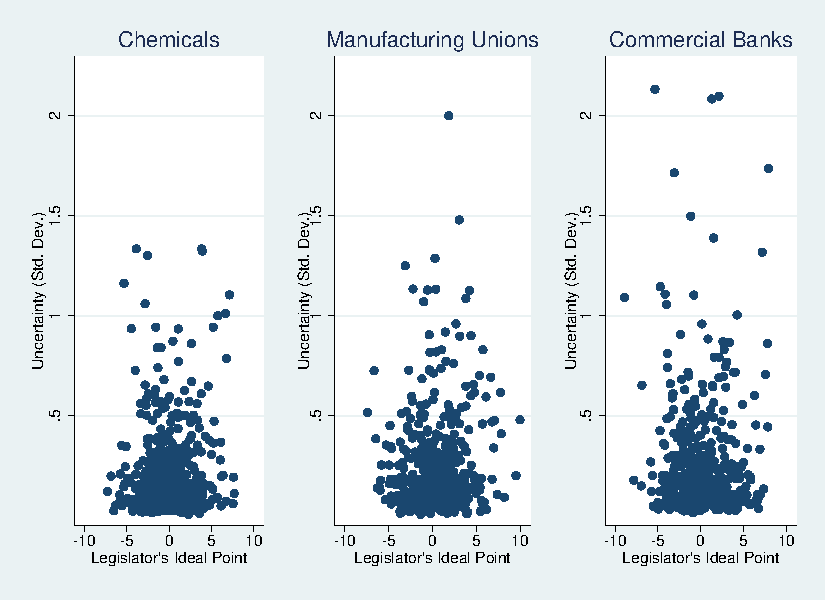
\includegraphics[height=3in, width=6.5in]{NSF_combined_graph.pdf}
\end{center}
\caption{Uncertainty by Industry\label{fig:combined}}
\end{figure}

\textcolor{blue}{We `turn on' the parameters for interest groups for each vote according to the data from Maplight, which includes a listing of the votes for which each interest group took a position. This produces estimates for how ``friendly'' or ``unfriendly'' each legislator is with respect to each interest group, as well as the unpredictability of his/her voting behavior when matters affecting that group are considered. In a preliminary run of this model with just ten interest groups (out of over 450) in the 112th Congress displayed in Figure~\ref{fig:combined}, we find that the chemical industry has the lowest average uncertainty (sd = 0.229); this is lower than the total uncertainty measure that can be interpreted as the standard left-right measure in ideal point models (sd = 0.233). The median group in terms of uncertainty is manufacturing unions (sd = 0.253), while construction equipment faced the highest uncertainty (sd = 0.285).}

\textcolor{blue}{We are experimenting with some of the more sophisticated measures of uncertainty that are possible with a rich model such as this one; for instance the group mean for $\ga$ and constructs that combine model parameters.}

\textcolor{blue}{Having created these measures of political uncertainty---which are entirely new to the best of our knowledge---we will proceed to characterize this uncertainty across industries, as well as how it is related to lobbying, political contributions and voting behavior of legislators. First, we want to understand the patterns in these data in the context of the industry-relevant bills identified by Maplight (as explained above).} 

\textcolor{blue}{We will use descriptive analysis as well as both standard parametric and non-parametric techniques such as density estimation to explore the relationships between the above variables of interest. We will begin with very basic questions such as whether distinct industries face varying levels of political uncertainty (see preliminary evidence in Figure~\ref{fig:combined}) and how those patterns may relate to the lobbying strategies they employ. From the data analysis that is represented above, we see a very interesting relationship between uncertainty and lobbying expenditure across legislators at the aggregate level in Figure~\ref{fig:br}, and we expect that additional important patterns will emerge when the data is disaggregated by industry.}



\section{An Application to the U.S. House of Representatives}
\label{sec:house}

\subsection{Data}
\textcolor{blue}{Voting data will be obtained from Vote View, a website maintained by Professor Keith Poole (\url{http://voteview.com}). Details on each legislative proposal are available electronically through Thomas (\url{http://thomas.loc.gov}) and the sites of the House and Senate registrars.}

\textcolor{blue}{We will use Maplight's contributions data, which provides evidence on public declarations by special interest groups to determine the relevant PAC contributions for the bills under consideration. In a related effort to better connect special interest activity to the intent of that activity, we will use data made available pursuant to the U.S. Lobbying Disclosure Act of 1995 and the Honest Leadership and Open Government Act of 2007 via the U.S. Senate Office of Public Records and the Office of the Clerk of the U.S. House of Representatives. This data is particularly useful because lobbyists must declare the issue area on which they lobbied.}

\textcolor{blue}{We will also explore whether there is a way to leverage the data and methodology of Lake and Millimet (2014b) that combine the contributions and lobbying data to improve precision, although there is a concern about the coarseness of the data that must be overcome.}

\subsection{Evidence}

\begin{figure}
\centering
\begin{minipage}{.5\textwidth}
  \centering
  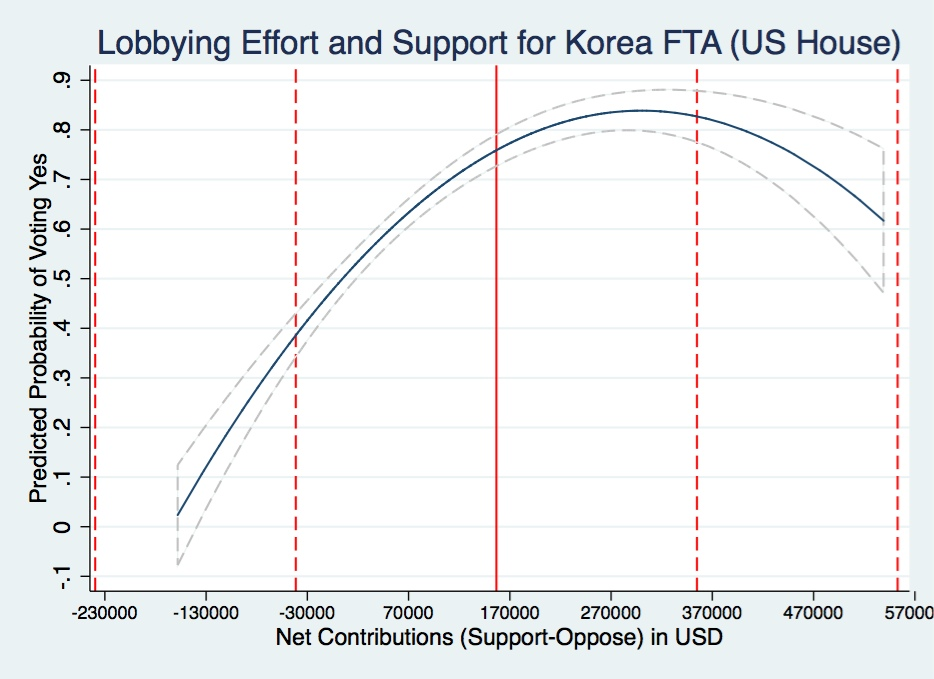
\includegraphics[width=2.9in]{graph2.jpg}
  \caption{Lobbying Effort and Support for KORUS
	\label{fig:br}}
\end{minipage}%
\begin{minipage}{.5\textwidth}
  \centering
  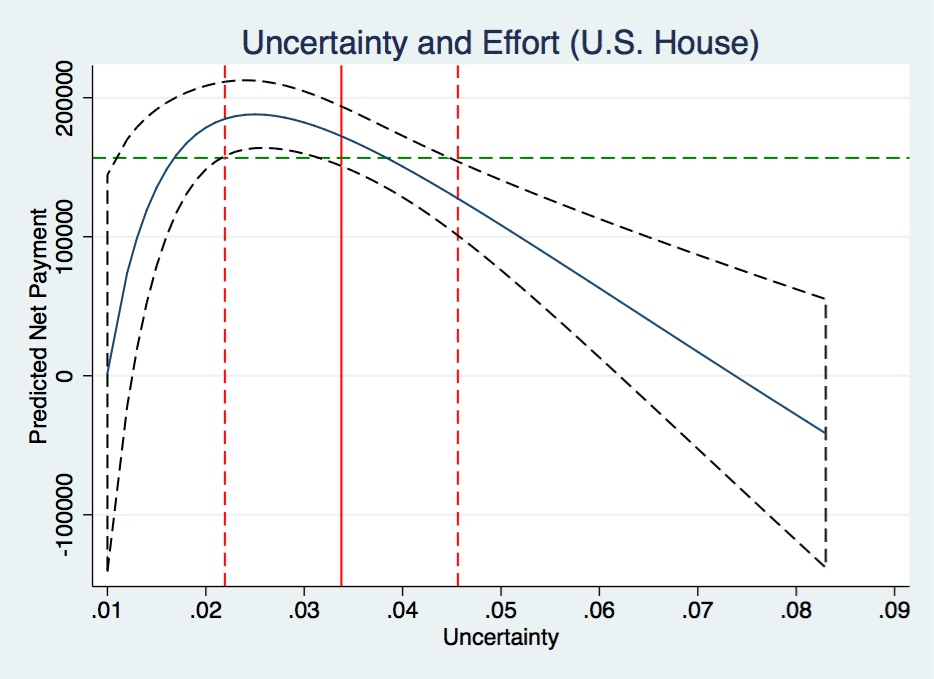
\includegraphics[width=2.9in]{graph1.jpg}
  \caption{Net Campaign Contributions, KORUS
	\label{fig:g1}}
\end{minipage}
\end{figure}

\textcolor{blue}{Figure~\ref{fig:br} displays the relationship between lobbying effort and legislators' support for KORUS. The vertical axis represents the predicted probability that a legislator would vote ``yes'' on the agreement, and the horizontal axis shows the monetary contributions to each legislator by lobbies who supported the passage of KORUS minus the contributions from lobbies opposing the agreement. The solid vertical red line indicates the average net contribution in the sample, and the dashed lines a one-standard deviation increase/decrease from that sample mean. The data indicate that exporting industries are more likely to exert lobbying effort to enlist the support of additional legislators (extensive margin) rather than secure stronger support from a given set of legislators (intensive margin), as well as that there are decreasing returns to lobbying effort. To generate these results,  we regressed a legislator's vote on his/her estimated ideal point as well as partisanship using a probit specification. Then we fitted a second-order polynomial to the predicted probabilities generated by the probit regression. The contribution data for both this and the follow figure was obtained from Maplight.}

\textcolor{blue}{Figure~\ref{fig:g1} displays the relationship between the unpredictability of legislators' voting behavior and lobbying effort. The vertical axis represents the predicted net contributions to members of the U.S. House of Representatives in 2012, and the horizontal axis shows the unpredictability of legislator's voting behavior measured using the 95$\%$ posterior confidence intervals of their ideal points estimated using Bayesian Markov chain simulation to scale all roll call votes taken in the 112th Congress (more details on the methodology below). The solid vertical red line indicates the average uncertainty in the sample, and the vertical dashed red lines indicate increases/decreases of one-standard deviation from the average. The horizontal dashed green line indicates the predicted net payment in the sample. The data show a very strong relationship between uncertainty at the level of the individual legislator and campaign contributions. To generate these results, we fitted a second-order polynomial to the data, and used monetary contributions to each legislator by lobbies who supported the passage of KORUS minus the contributions from lobbies opposing the agreement. While these data do not map perfectly onto our theoretical constructs, they indicate that there is strong preliminary support for our hypotheses making it highly likely that investment in data acquisition and analysis is worthwhile.}



%\subsection{Break Decision}

%\subsection{Uncertainty for Select Interest Groups}
%\label{sec:select}


\section{Conclusion}
\label{sec:concl}

\textcolor{blue}{an alternative characterization of the legislative process would be one in which (i) bills have a quality dimension (such as their technical merit, or their appropriateness for a given situation); and (ii) legislators have access to different pieces of information about the quality of these proposals. Given our own long-term research agenda, adding common values and decentralized information to the analysis of the ratification of trade agreements will be one of the next steps in this project. Given the important set of governance characteristics identified in Mansfield and Milner (2012), we also look forward to taking advantage of what seems a rich opportunity to integrate important institutional variations into this modeling framework of endogenous lobbying with uncertainty.}

\vskip.3in
\textcolor{blue}{We expect this data will have a wide array of applications, such as exploring the links between policy uncertainty, the business cycle, and stock market volatility.}

\section*{Appendix}

			




\newpage
\section*{References}

\begin{list}{}{\setlength{\leftmargin}{0.3in}\setlength{\rightmargin}{0.0in}\setlength{\itemindent}{-0.3in}\setlength{\itemsep}{0.0in}}


\item Ansolabehere, S., J. de Figueiredo, and J. Snyder Jr. (2003), ``Why Is There so Little Money in U.S. Politics?,'' {\em Journal of Economic Perspectives}, 17, 105-130.

\item Becker, G., (1983) ``A Theory of Competition among Interest Groups for Political Influence.'' {\em Quarterly Journal of Economics} 98, 371-400.

\item Bombardini, M. (2008), ``Firm Heterogeneity and Lobby Participation,'' {\em Journal of International Economics}, 75, 329-348.

\item Bombardini, M., and F. Trebbi (2012): ``Competition and Political Organization: Together or Alone in Lobbying for Trade Policy?'' {\em Journal of International Economics}, 87, 18-26.

\item Clinton, J., Jackman, S., and D. Rivers, (2004): ``The Statistical Analysis of Roll Call Data.'' {\em American Political Science Review}, 98, 355-370.

\item Dal Bo, E. (2007): ``Bribing Voters.'' {\em American Journal of Political Science} 51, 789-803.

\item Dekel, E., Jackson, M., Wolinsky, A. (2005): {\em Vote Buying.} Unpublished manuscript, Caltech.

\item Gawande, K., P. Krishna and M. Robbins (2006): ``Foreign Lobbies and U.S. Trade Policy,'' {\em Review of Economics and Statistics}, 88, 563-571.

\item Goldberg, P. and G. Maggi (1999): ``Protection for Sale: An Empirical Investigation,'' {\em American Economic Review}, 89, 1135-1155.

\item Groseclose, T., Snyder, J. M. (1996): ``Buying Supermajorities.'' {\em American Political Science Review} 90, 303-315.

\item Grossman, G. and E. Helpman (1994): ``Protection for Sale,'' {\em The American Economic Review}, 84, 833-850.

\item Grossman, G. and E. Helpman (2005): ``A Protectionist Bias in Majoritarian Politics,'' {\em The Quarterly Journal of Economics}, 120, 1239-1282.

\item Henisz, W. and E. Mansfield (2006), ``Votes and Vetoes: The Political Determinants of Commercial Openness,'' {\em International Studies Quarterly}, 50, 189-211.

\item Kibris, A. (2012), ``Uncertainty and Ratification Failure,'' {\em Public Choice}, 150, 439-467.

\item Laffont, J., Tirole, J. (1994): ``A Theory of Incentives in Procurement and Regulation.'' Cambridge: MIT Press.

\item Laver, M. and K. Shepsle (1991), ``Divided Government: America is Not `Exceptional','' {\em Governance: An International Journal of Policy and Administration}, 4, 250-269.

\item Le Breton, M. and F. Salanie (2003), ``Lobbying under political uncertainty,'' {\em Journal of Public Economics}, 87, 2589-2610.

\item Le Breton, M. and V. Zaporozhets (2007), ``Legislative Lobbying under Political Uncertainty,'' Available at SSRN: \url{http://ssrn.com/abstract=1024686}.

\item Peltzman, S. (1976), ``Toward a More General Theory of Regulation.'' {\em Journal of Law and Economics} 19, 211-248.

\item Poole, K. T. (2005), ``Spatial Models of Parliamentary Voting.'' New York: Cambridge University Press.

\item Saiegh, S. (2009), ``Political  Prowess or Lady Luck? Evaluating Chief Executives' Legislative Success Rates,'' {\em The Journal of Politics}, 71, 1342-1356.

\item Saiegh, S. (2011) ``Ruling by Statute: How Uncertainty and Vote-Buying Shape Lawmaking.'' New York: Cambridge University Press.

\item Stigler, G. (1975) ``The Citizen and the State: Essays on Regulation.'' Chicago: Chicago University Press.


\end{list}

\end{document}